% -*- TeX-engine: xetex; eval: (auto-fill-mode 0); eval: (visual-line-mode 1); -*-
% Compile with XeLaTeX

%%%%%%%%%%%%%%%%%%%%%%%
% Option 1: Slides: (comment for handouts)   %
%%%%%%%%%%%%%%%%%%%%%%%

%\documentclass[slidestop,compress,mathserif,12pt,t,professionalfonts,xcolor=table]{beamer}
%
%% solution stuff
%\newcommand{\solnMult}[1]{
%\only<1>{#1}
%\only<2->{\red{\textbf{#1}}}
%}
%\newcommand{\soln}[1]{\textit{#1}}

%%%%%%%%%%%%%%%%%%%%%%%%%%%%%%%
% Option 2: Handouts, without solutions (post before class)    %
%%%%%%%%%%%%%%%%%%%%%%%%%%%%%%%

 \documentclass[11pt,containsverbatim,handout,xcolor=xelatex,dvipsnames,table]{beamer}

 % handout layout
 \usepackage{pgfpages}
 \pgfpagesuselayout{4 on 1}[letterpaper,landscape,border shrink=5mm]

 % solution stuff
 \newcommand{\solnMult}[1]{#1}
 \newcommand{\soln}[1]{}

%%%%%%%%%%%%%%%%%%%%%%%%%%%%%%%%%%%%
% Option 3: Handouts, with solutions (may post after class if need be)    %
%%%%%%%%%%%%%%%%%%%%%%%%%%%%%%%%%%%%

% \documentclass[11pt,containsverbatim,handout,xcolor=xelatex,dvipsnames,table]{beamer}

% % handout layout
% \usepackage{pgfpages}
% \pgfpagesuselayout{4 on 1}[letterpaper,landscape,border shrink=5mm]

% % solution stuff
% \newcommand{\solnMult}[1]{\red{\textbf{#1}}}
% \newcommand{\soln}[1]{\textit{#1}}

%%%%%%%%%%%%%%%%%%%%%%%%%%%%%%%
% Option 4: Notes Only
%%%%%%%%%%%%%%%%%%%%%%%%%%%%%%%

% % See http://tex.stackexchange.com/questions/114219/add-notes-to-latex-beamer
% \documentclass[10pt,containsverbatim,xcolor=xelatex,dvipsnames,table,notes=only]{beamer}

% % handout layout
% \usepackage{pgfpages}
% \pgfpagesuselayout{2 on 1}[letterpaper, landscape, border shrink=5mm]

% % solution stuff
% \newcommand{\solnMult}[1]{#1}
% \newcommand{\soln}[1]{}

%%%%%%%%%%
% Load style file, defaults  %
%%%%%%%%%%

%%%%%%%%%%%%%%%%
% Themes
%%%%%%%%%%%%%%%%

% See http://deic.uab.es/~iblanes/beamer_gallery/ for mor options

% Style theme
\usetheme{Pittsburgh}

% Color theme
\usecolortheme{seahorse}

% Helvetica Neue Light for most text
\usepackage{fontspec}
\setsansfont{Helvetica Neue Light}

%%%%%%%%%%%%%%%%
% Packages
%%%%%%%%%%%%%%%%

\usepackage{geometry}
\usepackage{graphicx}
\usepackage{amssymb}
\usepackage{epstopdf}
\usepackage{amsmath}  	% this permits text in eqnarray among other benefits
\usepackage{url}		% produces hyperlinks
\usepackage[english]{babel}
\usepackage{colortbl}	% allows for color usage in tables
\usepackage{multirow}	% allows for rows that span multiple rows in tables
\usepackage{color}		% this package has a variety of color options
\usepackage{pgf}
\usepackage{calc}
\usepackage{ulem}
\usepackage{multicol}
\usepackage{textcomp}
\usepackage{listings}
\usepackage{changepage}
\usepackage{tikz}
\usetikzlibrary{trees}		% for probability trees
\usepackage{fancyvrb}	% for colored code chunks
\usepackage{nameref}

%%%%%%%%%%%%%%%%
% Remove navigation symbols
%%%%%%%%%%%%%%%%

\beamertemplatenavigationsymbolsempty
\hypersetup{pdfpagemode=UseNone} % don't show bookmarks on initial view

%%%%%%%%%%%%%%%%
% User defined colors
%%%%%%%%%%%%%%%%

% Pantone 2015 Spring colors
% http://iwork3.us/2014/09/16/pantone-2015-spring-fashion-report/
% update each semester or year

\xdefinecolor{custom_blue}{rgb}{0, 0.70, 0.79} % scuba blue
\xdefinecolor{custom_darkBlue}{rgb}{0.11, 0.31, 0.54} % classic blue
\xdefinecolor{custom_orange}{rgb}{0.97, 0.57, 0.34} % tangerine
\xdefinecolor{custom_green}{rgb}{0.49, 0.81, 0.71} % lucite green
\xdefinecolor{custom_red}{rgb}{0.58, 0.32, 0.32} % marsala

\xdefinecolor{custom_lightGray}{rgb}{0.78, 0.80, 0.80} % glacier gray
\xdefinecolor{custom_darkGray}{rgb}{0.54, 0.52, 0.53} % titanium

%%%%%%%%%%%%%%%%
% Template colors
%%%%%%%%%%%%%%%%

\setbeamercolor*{palette primary}{fg=white,bg= custom_blue}
\setbeamercolor*{palette secondary}{fg=black,bg= custom_blue!80!black}
\setbeamercolor*{palette tertiary}{fg=white,bg= custom_blue!80!black!80}
\setbeamercolor*{palette quaternary}{fg=white,bg= custom_blue}

\setbeamercolor{structure}{fg= custom_blue}
\setbeamercolor{frametitle}{bg= custom_blue!90}
\setbeamertemplate{blocks}[shadow=false]
\setbeamersize{text margin left=2em,text margin right=2em}

%%%%%%%%%%%%%%%%
% Styling fonts, bullets, etc.
%%%%%%%%%%%%%%%%

% title slide
\setbeamerfont{title}{size=\large,series=\bfseries}
\setbeamerfont{subtitle}{size=\large,series=\mdseries}
%\setbeamerfont{institute}{size=\large,series=\mdseries}

% color of alerted text
\setbeamercolor{alerted text}{fg=custom_orange}

% styling of itemize bullets
\setbeamercolor{item}{fg=custom_blue}
\setbeamertemplate{itemize item}{{{\small$\blacktriangleright$}}}
\setbeamercolor{subitem}{fg=custom_blue}
\setbeamertemplate{itemize subitem}{{\textendash}}
\setbeamerfont{itemize/enumerate subbody}{size=\footnotesize}
\setbeamerfont{itemize/enumerate subitem}{size=\footnotesize}

% styling of enumerate bullets
\setbeamertemplate{enumerate item}{\insertenumlabel.}
\setbeamerfont{enumerate item}{family={\fontspec{Helvetica Neue}}}
\setbeamerfont{enumerate subitem}{family={\fontspec{Helvetica Neue}}}
\setbeamerfont{enumerate subsubitem}{family={\fontspec{Helvetica Neue}}}

% make frame titles small to make room in the slide
\setbeamerfont{frametitle}{size=\small} 

% set Helvetica Neue font for frame and section titles
\setbeamerfont{frametitle}{family={\fontspec{Helvetica Neue}}}
\setbeamerfont{sectiontitle}{family={\fontspec{Helvetica Neue}}}
\setbeamerfont{section in toc}{family={\fontspec{Helvetica Neue}}}
\setbeamerfont{subsection in toc}{family={\fontspec{Helvetica Neue}}, size=\small}
\setbeamerfont{footline}{family={\fontspec{Helvetica Neue}}}
\setbeamerfont{subsection in toc}{family={\fontspec{Helvetica Neue}}}
\setbeamerfont{block title}{family={\fontspec{Helvetica Neue}}}

%%%%%%%%%%%%%%%%
% New fonts accessed by fontspec package
%%%%%%%%%%%%%%%%

% Monaco font for code
\newfontfamily{\monaco}{Monaco}

%%%%%%%%%%%%%%%%
% Color text commands
%%%%%%%%%%%%%%%%

%orange
\newcommand{\orange}[1]{\textit{\textcolor{custom_orange}{#1}}}

% yellow
\newcommand{\yellow}[1]{\textit{\textcolor{yellow}{#1}}}

% blue
\newcommand{\blue}[1]{\textit{\textcolor{blue}{#1}}}

% green
\newcommand{\green}[1]{\textit{\textcolor{custom_green}{#1}}}

% red
\newcommand{\red}[1]{\textit{\textcolor{custom_red}{#1}}}

% dark gray
\newcommand{\darkgray}[1]{\textit{\textcolor{custom_darkGray}{#1}}}

% light gray
\newcommand{\lightgray}[1]{\textit{\textcolor{custom_lightGray}{#1}}}

% pink
\newcommand{\pink}[1]{\textit{\textcolor{pink}{#1}}}


%%%%%%%%%%%%%%%%
% Custom commands
%%%%%%%%%%%%%%%%

% empty box for probability tree frame
\newcommand{\emptybox}[2]{
	\fbox{ \begin{minipage}{#1} \hfill\vspace{#2} \end{minipage} }
}

% cancel
\newcommand{\cancel}[1]{%
    \tikz[baseline=(tocancel.base)]{
        \node[inner sep=0pt,outer sep=0pt] (tocancel) {#1};
        \draw[red, line width=0.5mm] (tocancel.south west) -- (tocancel.north east);
    }%
}

% degree
\newcommand{\degree}{\ensuremath{^\circ}}

% cite
\newcommand{\ct}[1]{
\vfill
{\tiny #1}}

% Note
\newcommand{\Note}[1]{
\rule{2.5cm}{0.25pt} \\ \textit{\footnotesize{\textcolor{custom_red}{Note:} \textcolor{custom_darkGray}{#1}}}}

% Remember
\newcommand{\Remember}[1]{\textit{\scriptsize{\textcolor{custom_red}{Remember:} #1}}}

% links: webURL, webLink
\newcommand{\webURL}[1]{\urlstyle{same}{\textit{\textcolor{custom_blue}{\url{#1}}}}}
\newcommand{\webLink}[2]{\href{#1}{\textcolor{custom_blue}{{#2}}}}

% mail
\newcommand{\mail}[1]{\href{mailto:#1}{\textit{\textcolor{custom_blue}{#1}}}}

% highlighting: hl, hlGr, mathhl
\newcommand{\hl}[1]{\textit{\textcolor{custom_blue}{#1}}}
\newcommand{\hlGr}[1]{\textit{\textcolor{custom_green}{#1}}}
\newcommand{\mathhl}[1]{\textcolor{custom_blue}{\ensuremath{#1}}}

% example
\newcommand{\ex}[1]{\textcolor{blue}{{{\small (#1)}}}}

% two col: two columns
\newenvironment{twocol}[4]{
\begin{columns}[c]
\column{#1\textwidth}
#3
\column{#2\textwidth}
#4
\end{columns}
}

% slot (for probability calculations)
\newenvironment{slot}[2]{
\begin{array}{c} 
\underline{#1} \\ 
#2
\end{array}
}

% pr: left and right parentheses
\newcommand{\pr}[1]{
\left( #1 \right)
}

%%%%%%%%%%%%%%%%
% Custom blocks
%%%%%%%%%%%%%%%%

% activity: less commonly used
\newcommand{\activity}[2]{
\setbeamertemplate{itemize item}{{{\small\textcolor{custom_orange}{$\blacktriangleright$}}}}
\setbeamercolor{block title}{fg=white, bg=custom_orange}
\setbeamerfont{block title}{size=\small}
\setbeamercolor{block body}{fg=black, bg=custom_orange!20!white!80}
\setbeamerfont{block body}{size=\small}
\begin{block}{Activity: #1}
\setlength\abovedisplayskip{0pt}
#2
\end{block}
}

% app: application exercise
\newcommand{\app}[2]{
\setbeamercolor{block title}{fg=white,bg=custom_green}
\setbeamercolor{block body}{fg=black,bg=custom_green!20!white!80}
\begin{block}{{\small Application exercise: #1}}
#2
\end{block}
}

% disc: discussion question
\newcommand{\disc}[1]{
\vspace*{-2ex}
\setbeamercolor{block body}{bg=custom_blue!25!white!80, fg=custom_blue!55!black!95}
\begin{block}{\vspace*{-3ex}}
#1
\end{block}
\vspace*{-1ex}
}

% clicker: clicker question
\newcommand{\clicker}[1]{
\setbeamercolor{block title}{bg=custom_blue!80!white!50,fg=custom_blue!30!black!90}
\setbeamercolor{block body}{bg=custom_blue!20!white!80,fg=custom_blue!30!black!90}
\begin{block}{\vspace*{-0.2ex}{\footnotesize Clicker question}\vspace*{-0.2ex}}
#1
\end{block}
}

% formula
\newcommand{\formula}[2]{
\setbeamercolor{block title}{bg=custom_blue!40!white!60,fg=custom_blue!55!black!95}
\begin{block}{{\small#1}}
#2
\end{block}
}

% code
\newcommand{\Rcode}[1]{
{\monaco {\footnotesize \textcolor{custom_darkBlue}{#1}}}
}

% output
\newcommand{\Rout}[1]{
{\monaco {\footnotesize \textcolor{custom_darkGray}{#1}}}
}

%%%%%%%%%%%%%%%%
% Change margin
%%%%%%%%%%%%%%%%

\newenvironment{changemargin}[2]{%
\begin{list}{}{%
\setlength{\topsep}{0pt}%
\setlength{\leftmargin}{#1}%
\setlength{\rightmargin}{#2}%
\setlength{\listparindent}{\parindent}%
\setlength{\itemindent}{\parindent}%
\setlength{\parsep}{\parskip}%
}%
\item}{\end{list}}

%%%%%%%%%%%%%%%%
% Footnote
%%%%%%%%%%%%%%%%

\long\def\symbolfootnote[#1]#2{\begingroup%
\def\thefootnote{\fnsymbol{footnote}}\footnote[#1]{#2}\endgroup}

%%%%%%%%%%%%%%%%
% Graphics
%%%%%%%%%%%%%%%%

\DeclareGraphicsRule{.tif}{png}{.png}{`convert #1 `dirname #1`/`basename #1 .tif`.png}

%%%%%%%%%%%%%%%%
% Slide number
%%%%%%%%%%%%%%%%

\setbeamertemplate{footline}{%
    \raisebox{5pt}{\makebox[\paperwidth]{\hfill\makebox[20pt]{\color{gray}
          \scriptsize\insertframenumber}}}\hspace*{5pt}}

          
%%%%%%%%%%%%%%%%
% Remove page numbers
%%%%%%%%%%%%%%%%

\newcommand{\removepagenumbers}{% 
  \setbeamertemplate{footline}{}
}

%%%%%%%%%%%%%%%%
% TOC slides
%%%%%%%%%%%%%%%%

\setbeamertemplate{section in toc}{\inserttocsectionnumber.~\inserttocsection}
\setbeamertemplate{subsection in toc}{$\qquad$\inserttocsubsectionnumber.~\inserttocsubsection \\}

\AtBeginSection[] 
{ 
  \addtocounter{framenumber}{-1} 
  % 
  {\removepagenumbers 
  {\small
    \begin{frame}<beamer> 
    \frametitle{Outline} 
    \tableofcontents[currentsection] 
  \end{frame} 
  } 
  }
} 

\AtBeginSubsection[] 
{ 
  \addtocounter{framenumber}{-1} 
  % 
  {\removepagenumbers 
  {\small
    \begin{frame}<beamer> 
    \frametitle{Outline} 
    \tableofcontents[currentsection,currentsubsection] 
  \end{frame} 
  } 
  }
}
% You cannot use numbers when defining variables.  Hence the use of letters, A, B, C, etc.

% Personal Info
\newcommand{\FirstName}{Mine}
\newcommand{\LastName}{\c{C}etinkaya-Rundel}
\newcommand{\OfficeHours}{Generally TR 12:30 - 1:30pm}

% Electronic Info
\newcommand{\PersonalSite}{http://stat.duke.edu/~mc301}
\newcommand{\CourseSite}{http://bit.ly/sta104su15}
\newcommand{\Email}{mine@stat.duke.edu}

% TAs
\newcommand{\TAA}{Andrew Wong}

% Exam Dates
\newcommand{\ExamDate}{May 29, 11am - 12:30pm (in class)}
\newcommand{\FinalDate}{June 24, 11am - 2pm}

% ALT ALT
% \input{../../definitions_custom.tex}

%%%%%%%%%%%
% Cover slide info    %
%%%%%%%%%%%

\title{Unit 4: Inference for numerical data}
\subtitle{2. Bootstrapping + Comparing means}
\author{Sta 104 - Summer 2015}
\date{June 2, 2015}
\institute{Duke University, Department of Statistical Science}

%%%%%%%%%%%%%%%%%%%%%%%%%
% Begin document and set Helvetica Neue font   %
%%%%%%%%%%%%%%%%%%%%%%%%%

\begin{document}
\fontspec[Ligatures=TeX]{Helvetica Neue Light}

%%%%%%%%%%%%%%%%%%%%%%%%%%%%%%%%%%%

% Title Page

\begin{frame}[plain]

\titlepage
\vfill
{\scriptsize \webLink{\PersonalSite}{Dr. \LastName{}} \hfill Slides posted at  \webLink{\CourseSite}{\CourseSite}}
\addtocounter{framenumber}{-1} 

\end{frame}

%%%%%%%%%%%%%%%%%%%%%%%%%%%%%%%%%%%

\section{Housekeeping}

%%%%%%%%%%%%%%%%%%%%%%%%%%%%%%%%%%%

\begin{frame}
\frametitle{Announcements}

\begin{itemize}

\item 

\end{itemize}

\end{frame}

%%%%%%%%%%%%%%%%%%%%%%%%%%%%%%%%%%%

\section{Main ideas - Bootstrapping}

%%%%%%%%%%%%%%%%%%%%%%%%%%%%%%%%%%%

\subsection{Bootstrap to a confidence interval for any parameter via simulation}
\label{mi1boot}

%%%%%%%%%%%%%%%%%%%%%%%%%%%%%%%%%%%

\begin{frame}
\frametitle{Rotten horrors}

\twocol{0.4}{0.6}
{

\includegraphics[width = 0.8\textwidth]{figures/movies/rotten_tomatoes} \\
is a movie aggregator, where the audience is also able to review and score the movies. We want to estimate the average audience score of horror movies on RottenTomatoes.com. We start with a random sample of 20 horror movies.
}
{
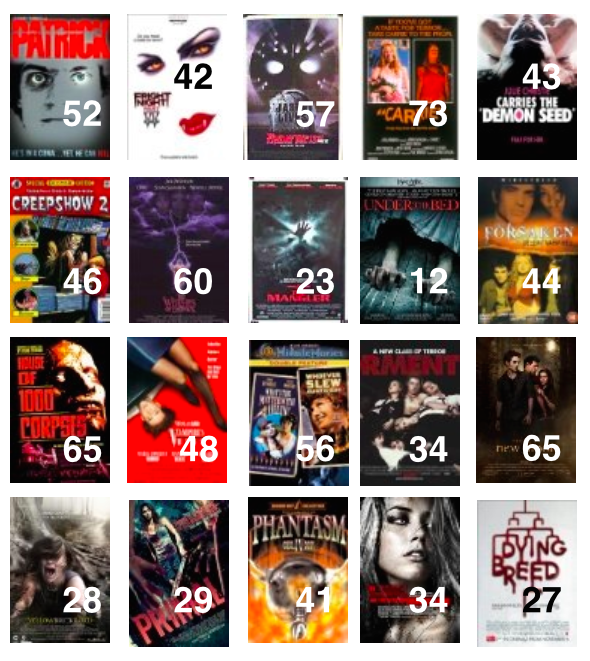
\includegraphics[width = \textwidth]{figures/movies/horror_data}
}

\end{frame}

%%%%%%%%%%%%%%%%%%%%%%%%%%%%%%%%%%%

\begin{frame}[fragile]
\frametitle{Data}

{\scriptsize
\begin{verbatim}
                                  title audience_score
 1                              Patrick             52
 2                           Demon Seed             43
 3                            Tormented             34
 4                        Under the Bed             12
 5                Phantasm IV: Oblivion             41
 6                  Fright Night Part 2             42
 7                House of 1000 Corpses             65
 8                          Creepshow 2             46
 9                         The Forsaken             44
10         All the Boys Love Mandy Lane             34
11 Jason Lives: Friday the 13th Part VI             57
12                       Vampire's Kiss             48
13              The Witches of Eastwick             60
14                      Yellowbrickroad             28
15                          Dying Breed             27
16                               Carrie             73
17             Whoever Slew Auntie Roo?             56
18                          The Mangler             23
19                               Primal             29
20          The Twilight Saga: New Moon             65
\end{verbatim}
}

\end{frame}

%%%%%%%%%%%%%%%%%%%%%%%%%%%%%%%%%%%

\begin{frame}
\frametitle{First look}

\disc{{\small The histogram below shows the distribution of the audience scores of these movies (ranging from 0 to 100). The median score in the sample is 43.5. Can we apply CLT based methods we have learned so far to construct a confidence interval for the \underline{median} RottenTomatoes score of horror movies. Why or why not?}}

\begin{center}
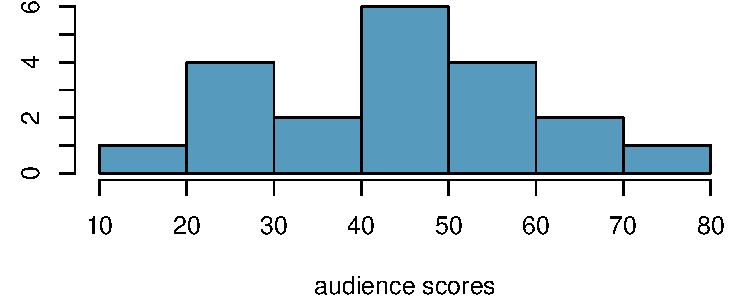
\includegraphics[width = 0.8\textwidth]{figures/movies/horror_hist}
\end{center}

\end{frame}

%%%%%%%%%%%%%%%%%%%%%%%%%%%%%%%%%%%

\begin{frame}
\frametitle{Bootstrapping}

\begin{itemize}

\item An alternative approach to constructing confidence intervals is \hl{bootstrapping}. 

\pause

\item This term comes from the phrase ``pulling oneself up by one's bootstraps", which is a metaphor for accomplishing an impossible task without any outside help. 

\pause

\item In this case the \sout{im}possible task is estimating a population parameter, and we'll accomplish it using data from only the given sample.

\end{itemize}

\hfill 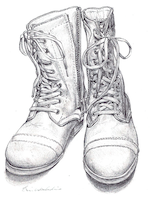
\includegraphics[width = 0.25\textwidth]{figures/boot}

\end{frame}

%%%%%%%%%%%%%%%%%%%%%%%%%%%%%%%%%%%%%

\begin{frame}
\frametitle{Bootstrapping}

\begin{itemize}

\item Bootstrapping works as follows:
\pause
\begin{enumerate}[(1)]
\item take a bootstrap sample - a random sample taken with replacement from the original sample, of the same size as the original sample
\pause
\item calculate the bootstrap statistic - a statistic such as mean, median, proportion, etc. computed on the bootstrap samples
\pause
\item repeat steps (1) and (2) many times to create a bootstrap distribution - a distribution of bootstrap statistics
\end{enumerate}

\pause

\item The XX\% bootstrap confidence interval can be estimated by
\begin{itemize}
\pause
\item the cutoff values for the middle XX\% of the bootstrap distribution,
\item[]
\pause
\item[] OR
\item[]
\pause
\item $\bar{x}_{boot} \pm z^\star SE_{boot}$
\end{itemize}

\end{itemize}

\end{frame}

%%%%%%%%%%%%%%%%%%%%%%%%%%%%%%%%%%%%%

\begin{frame}[fragile]
\frametitle{Bootstrap sample 1}

{\small \textbf{(1) Take a bootstrap sample:}}
\pause
{\tiny
\begin{verbatim}
                                  title audience_score
 1                       Vampire's Kiss             48
 2                Phantasm IV: Oblivion             41
 3                House of 1000 Corpses             65
 4                          Dying Breed             27
 5             Whoever Slew Auntie Roo?             56
 6                         The Forsaken             44
 7          The Twilight Saga: New Moon             65
 8          The Twilight Saga: New Moon             65
 9             Whoever Slew Auntie Roo?             56
10          The Twilight Saga: New Moon             65
11                          The Mangler             23
12                          Dying Breed             27
13                          Creepshow 2             46
14                House of 1000 Corpses             65
15             Whoever Slew Auntie Roo?             56
16                            Tormented             34
17 Jason Lives: Friday the 13th Part VI             57
18                       Vampire's Kiss             48
19                               Primal             29
20              The Witches of Eastwick             60
\end{verbatim}
}

\pause

{\small \textbf{(2) Calculate the median of the bootstrap sample:}} \\
\pause
{\footnotesize
23, 27, 27, 29, 34, 41, 44, 46, 48, \red{48, 56}, 56, 56, 57, 60, 65, 65, 65, 65, 65 \\
median = (48 + 56) / 2 = 52 \\
}

\pause

{\small
\textbf{(3) Record this value}
}

\end{frame}

%%%%%%%%%%%%%%%%%%%%%%%%%%%%%%%%%%%%%

\begin{frame}[fragile]
\frametitle{Bootstrap sample 2}

{\small \textbf{(1) Take another bootstrap sample:}}
\pause
{\tiny
\begin{verbatim}
                                  title audience_score
 1                  Fright Night Part 2             42
 2                               Carrie             73
 3                         The Forsaken             44
 4                          The Mangler             23
 5                               Primal             29
 6                              Patrick             52
 7 Jason Lives: Friday the 13th Part VI             57
 8                          The Mangler             23
 9                       Vampire's Kiss             48
10         All the Boys Love Mandy Lane             34
11          The Twilight Saga: New Moon             65
12         All the Boys Love Mandy Lane             34
13                      Yellowbrickroad             28
14                       Vampire's Kiss             48
15                            Tormented             34
16                          The Mangler             23
17                Phantasm IV: Oblivion             41
18                              Patrick             52
19                House of 1000 Corpses             65
20          The Twilight Saga: New Moon             65
\end{verbatim}
}

\pause

{\small \textbf{(2) Calculate the median of the bootstrap sample:}} \\
\pause
{\footnotesize
23, 23, 23, 28, 29, 34, 34, 34, 41, \red{42, 44}, 48, 48, 52, 52, 57, 65, 65, 65, 73 \\
median = (42 + 44) / 2 = 43 \\
}

\pause

{\small
\textbf{(3) Record this value}
}

\end{frame}

%%%%%%%%%%%%%%%%%%%%%%%%%%%%%%%%%%%%%

\begin{frame}[fragile]
\frametitle{Bootstrap sample 3}

{\small \textbf{(1) Take another bootstrap sample:}}
\pause
{\tiny
\begin{verbatim}
                                  title audience_score
 1                            Tormented             34
 2              The Witches of Eastwick             60
 3              The Witches of Eastwick             60
 4              The Witches of Eastwick             60
 5                          The Mangler             23
 6              The Witches of Eastwick             60
 7                              Patrick             52
 8                Phantasm IV: Oblivion             41
 9                      Yellowbrickroad             28
10 Jason Lives: Friday the 13th Part VI             57
11                      Yellowbrickroad             28
12 Jason Lives: Friday the 13th Part VI             57
13                  Fright Night Part 2             42
14                               Primal             29
15                  Fright Night Part 2             42
16             Whoever Slew Auntie Roo?             56
17                  Fright Night Part 2             42
18                  Fright Night Part 2             42
19                        Under the Bed             12
20                Phantasm IV: Oblivion             41
\end{verbatim}
}

\pause

{\small \textbf{(2) Calculate the median of the bootstrap sample:}} \\
\pause
{\footnotesize
12, 23, 28, 28, 29, 34, 41, 41, 42, \red{42, 42}, 42, 52, 56, 57, 57, 60, 60, 60, 60 \\
median = (42 + 42) / 2 = 42 \\
}

\pause

{\small
\textbf{(3) Record this value}
}

\end{frame}

%%%%%%%%%%%%%%%%%%%%%%%%%%%%%%%%%%%%%

\begin{frame}
\frametitle{Many more bootstrap samples}

\vfill

... repeat

\vfill

\end{frame}

%%%%%%%%%%%%%%%%%%%%%%%%%%%%%%%%%%%%%

\begin{frame}
\frametitle{}

\clicker{The dot plot  below is the bootstrap distribution of medians constructed using 100 simulations. What does each dot on the dot plot represent?}

\begin{center}
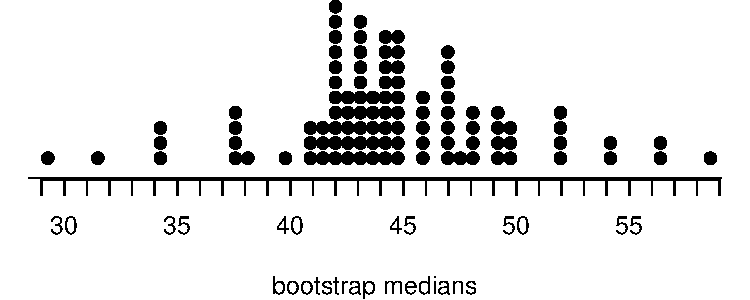
\includegraphics[width = 0.6\textwidth]{figures/movies/horror_boot_med_dot}
\end{center}

\begin{enumerate}[(a)]
\item Score of a horror movie in the original sample
\item Score of a horror movie in the population
\item \solnMult{Median from one bootstrap sample from the original sample}
\item Median from one sample from the population
\end{enumerate}

\end{frame}

%%%%%%%%%%%%%%%%%%%%%%%%%%%%%%%%%%

\begin{frame}
\frametitle{}

\clicker{The dot plot  below shows the distribution of 100 bootstrap medians. Estimate the 90\% bootstrap confidence interval for the median RT score of horror movies using the percentile method.}

\only<1>{
\begin{center}
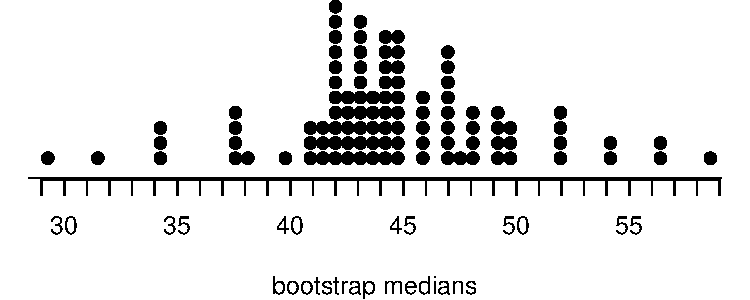
\includegraphics[width = 0.8\textwidth]{figures/movies/horror_boot_med_dot}
\end{center}
}

\soln{\only<2->{
\begin{center}
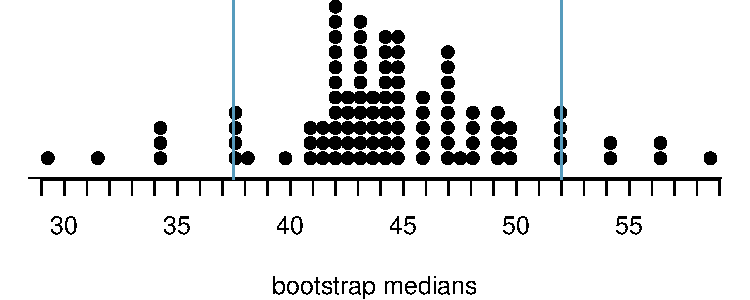
\includegraphics[width = 0.8\textwidth]{figures/movies/horror_boot_med_dot_soln}
\end{center}
}}

\begin{multicols}{2}
\begin{enumerate}[(a)]
\item (29, 58.5)
\item (34, 57)
\item \solnMult{(37.5, 52)}
\item (40, 49.5)
\end{enumerate}
\end{multicols}

\end{frame}

%%%%%%%%%%%%%%%%%%%%%%%%%%%%%%%%%

\begin{frame}
\frametitle{Botstrap interval, standard error}

\disc{The dot plot  below shows the distribution of 100 bootstrap medians. The median of the original sample is 43.5 and the bootstrap standard error is 4.88. Estimate the 90\% bootstrap confidence interval for the median RT score of horror movies using the standard error method.}

\begin{center}
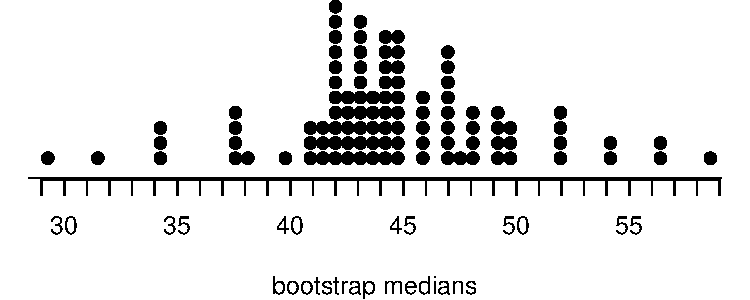
\includegraphics[width = 0.75\textwidth]{figures/movies/horror_boot_med_dot}
\end{center}

\pause

\soln{\[ 43.5 \pm (1.65 \times 4.88) = (35.45, 51.55) \] }

\end{frame}

%%%%%%%%%%%%%%%%%%%%%%%%%%%%%%%%%

\begin{frame}
\frametitle{Bootstrap vs. sampling distributions}

\vfill

\app{4.2 Bootstrap intervals}{See the course webpage for details.}

\vfill

\end{frame}

%%%%%%%%%%%%%%%%%%%%%%%%%%%%%%%%%%

\subsection{Bootstrap, but center at the null, for testing for a single parameter}
\label{mi2boot}

%%%%%%%%%%%%%%%%%%%%%%%%%%%%%%%%%%%

\begin{frame}
\frametitle{Bootstrap testing for a mean}

\begin{itemize}

\item This is very similar to bootstrapping, i.e. we randomly sample with replacement from the sample, but this time we shift the bootstrap distribution to be \underline{centered at the null value}. 

\pause

\item The p-value is then defined as the proportion of simulations that yield a sample statistic at least as favorable to the alternative hypothesis as the observed sample statistic.

\end{itemize}

\end{frame}

%%%%%%%%%%%%%%%%%%%%%%%%%%%%%%%%%%%

\begin{frame}
\frametitle{}

\disc{Do these data provide convincing evidence that the median audience score of horror movies is greater than 40? Remember that the median of the original sample was 43.5.}

\begin{center}
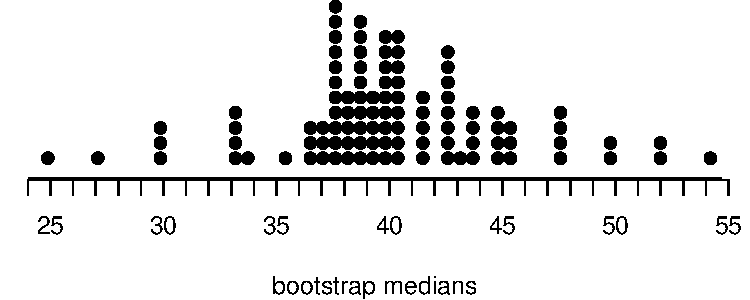
\includegraphics[width = 0.75\textwidth]{figures/movies/horror_boot_med_test_dot}
\end{center}

\pause

\twocol{0.3}{0.7}{
\begin{itemize}
\item[$H_0:$] $median = 40$
\item[$H_A:$] $median > 40$
\end{itemize}
}
{
\pause
p-value: proportion of simulations where the simulated bootstrap sample median is at least as extreme as the one observed (43.5). $\rightarrow$ 20 / 100 = 0.20
}

\end{frame}

%%%%%%%%%%%%%%%%%%%%%%%%%%%%%%%%%%%

\subsection{Recap}

%%%%%%%%%%%%%%%%%%%%%%%%%%%%%%%%%%%

\begin{frame}
\frametitle{}

\disc{Describe how you would construct a bootstrap interval for a proportion.}

\end{frame}

%%%%%%%%%%%%%%%%%%%%%%%%%%%%%%%%%%%

\subsection{Summary}

%%%%%%%%%%%%%%%%%%%%%%%%%%%%%%%%%%%

\begin{frame}
\frametitle{Summary of main ideas - Bootstrapping}

\vfill

\begin{enumerate}

\item \nameref{mi1boot}

\item \nameref{mi2boot}

\end{enumerate}

\vfill

\end{frame}

%%%%%%%%%%%%%%%%%%%%%%%%%%%%%%%%%%

\section{Main ideas - Comparing means}

%%%%%%%%%%%%%%%%%%%%%%%%%%%%%%%%%%

\subsection{When comparing means of two groups, ask if paired or independent}
\label{mi1}

%%%%%%%%%%%%%%%%%%%%%%%%%%%%%%%%%%%%

\begin{frame}
\frametitle{1. When comparing means of two groups, ask if paired or independent}

\begin{itemize}

\item dependent (paired) groups (e.g. pre/post weights of subjects in a weight loss study, twin studies, etc.)
\[ SE_{\bar{x}_{diff}} = \frac{s_{diff}}{\sqrt{n_{diff}}} \]

\item independent groups (e.g. grades of students across two sections)
\[ SE_{\bar{x}_1 - \bar{x}_2} = \sqrt{ \frac{s_1^2}{n_1} + \frac{s_2^2}{n_2} } \]

\end{itemize}

%---Note---%
\note{

- Go through some examples of where you have two groups.
  - Twin studies for instance.

- Overall SE increases when looking at two different groups.

- Lemonade and cup.  Uncertainty in both.  Makes uncertainty in difference
greater.

- Comment on types of data.

}

\end{frame}

%%%%%%%%%%%%%%%%%%%%%%%%%%%%%%%%%%%%

\subsection{T corrects for uncertainty introduced by plugging in $s$ for $\sigma$}
\label{mi2}

%%%%%%%%%%%%%%%%%%%%%%%%%%%%%%%%%%%%

\begin{frame}
\frametitle{2. T corrects for uncertainty introduced by plugging in $s$ for $\sigma$}

\begin{itemize}

\item Essential when $n$ is small ($n < 30$) since $s$ is more likely to be not be a good estimate for $\sigma$ when $n$ is small than when $n$ is large

\pause

\item Could be used when $n$ is large as well

\pause

\item Also has a bell shape, but its tails are \hl{thicker} than the normal model's
\begin{itemize}
\item Observations are more likely to fall beyond two SDs from the mean than under the normal distribution.
\end{itemize}

\pause

\item Extra thick tails are helpful for mitigating the effect of a less reliable estimate for the standard error of the sampling distribution (since $n$ is small)

\end{itemize}

\begin{center}
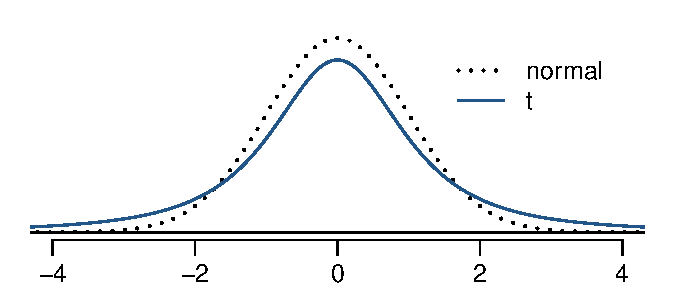
\includegraphics[width=0.5\textwidth]{figures/tDistCompareToNormalDist/tDistCompareToNormalDist}
\end{center}

%---Note---%
\note{

- Corrects for certainty when plugging in $s$ for $\sigma$.

- Question from student: when would you ever have small $n$?

- Think about squishing down distribution.

- Go through shape, center, symmetry, etc.

}

\end{frame}

%%%%%%%%%%%%%%%%%%%%%%%%%%%%%%%%%%%%

\begin{frame}
\frametitle{T distribution}

\begin{itemize}

\item Always centered at zero, like the standard normal ($z$) distribution

\pause

\item Has a single parameter: \hl{degrees of freedom} (\mathhl{df})
\begin{itemize}
\item one sample: $df = n - 1$
\item two (independent) samples: $df = min(n_1 - 1, n_2 - 1)$
\end{itemize}

\end{itemize}

\begin{center}
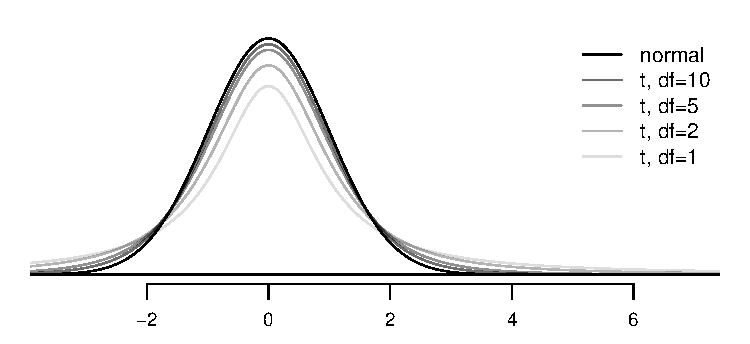
\includegraphics[width=0.8\textwidth]{figures/tDistConvergeToNormalDist/tDistConvergeToNormalDist}
\end{center}

\pause

\disc{What happens to shape of the T distribution as $df$ increases?}

\soln{\pause Approaches normal.}

\end{frame}

%%%%%%%%%%%%%%%%%%%%%%%%%%%%%%%%%%%%

\begin{frame}

\clicker{Under the T distribution with 5 degrees freedom, \_\_\_\_\_\_\_\_\_\_ of the data are within one standard deviation of the mean?}

\begin{enumerate}[(a)]
\item 68\%
\item \solnMult{less than 68\%}
\item more than 68\%
\end{enumerate}

\end{frame}

%%%%%%%%%%%%%%%%%%%%%%%%%%%%%%%%%%%%

\begin{frame}
\frametitle{}

\vfill

\app{4.3 Comparing means, Pt 1}{See the course webpage for details.}

\vfill

\end{frame}

%%%%%%%%%%%%%%%%%%%%%%%%%%%%%%%%%%

\begin{frame}
\frametitle{}

\vfill

\app{4.4 Comparing means, Pt 2}{See the course webpage for details.}

\vfill

\end{frame}

%%%%%%%%%%%%%%%%%%%%%%%%%%%%%%%%%%

\subsection{Summary}

%%%%%%%%%%%%%%%%%%%%%%%%%%%%%%%%%%%%

\begin{frame}
\frametitle{Summary of main ideas - comparing means}

\vfill

\begin{enumerate}

\item \nameref{mi1}

\item \nameref{mi2}

\end{enumerate}

\vfill

\end{frame}

%%%%%%%%%%%%%%%%%%%%%%%%%%%%%%%%%%%

\end{document}